\documentclass[../main.tex]{subfiles}

\begin{document}
A B\'ezier curve is a parametric curve used to model smooth curves.  In order to develop the sea floor map (without having to define every single point), we decided to use a cubic B\'ezier Curve.  A cubic B\'ezier curve takes in 4 control points and interpolates along the 4 points to develop a smooth, continuous curve.  The control points are defined as two points at the ends, one at $\frac{1}{3}$ of the way, and another at $\frac{2}{3}$ of the way.  Now, provided the control points, we have the following explicit form:
\begin{equation} \label{eq:bezier}
B(t) = (1-t)^3P_0 + 3t(1-t)^2P_1 + 3t^2(1-t)P_2+t^3P_3, \ \ \ \ 0\leq t \leq 1
\end{equation}
Where $P$ is the control point. We can use this explicit form to find the derivative at any point $t$:
\begin{equation}\label{eq:bezierderiv}
B'(t) = 3(1-t)^2(P_1-P_0) + 6t(1-t)(P_2-P_1) + 3t^2(P_3-P_2), \ \ \ \ 0\leq t \leq 1
\end{equation}
We can extend the idea of a B\'ezier curve to develop a B\'ezier surface, which is a 2D linearly interpolated surface that is made using 16 control points. The 16 control points create a $4 \times 4$ grid of points.  In order to find a single point on the surface, say $(u, v)$, we first create 4 new points by evaluating \eqref{eq:bezier} at $u$ using 4 sets of 4 control points.  That is, we calculate $B(u)$ using control points 1 through 4, then 5 through 8, 9 through 12, and finally 13
through 16.  We then use the 4 values of $B(u)$ as control points, and evaluate $B(v)$ to finally find the point on surface $(u, v)$.  This method is repeated on all points on the grid, in order to create the B\'ezier surface. 

\subsection{Implementation}
For our application with the Fukushima Daiichi Nuclear Power Plant, we derived the 4 control points for the sea floor using the National Oceanic and Atmospheric Administration's (NOAA) Bathymetric Data Viewer.  The viewer allows users to gain elevation data at any coordinate.  Thus, we drew a line between the epicenter of the earthquake to the nuclear power plant, and derived the 4 control points from there.
\begin{figure}[H]
\centering
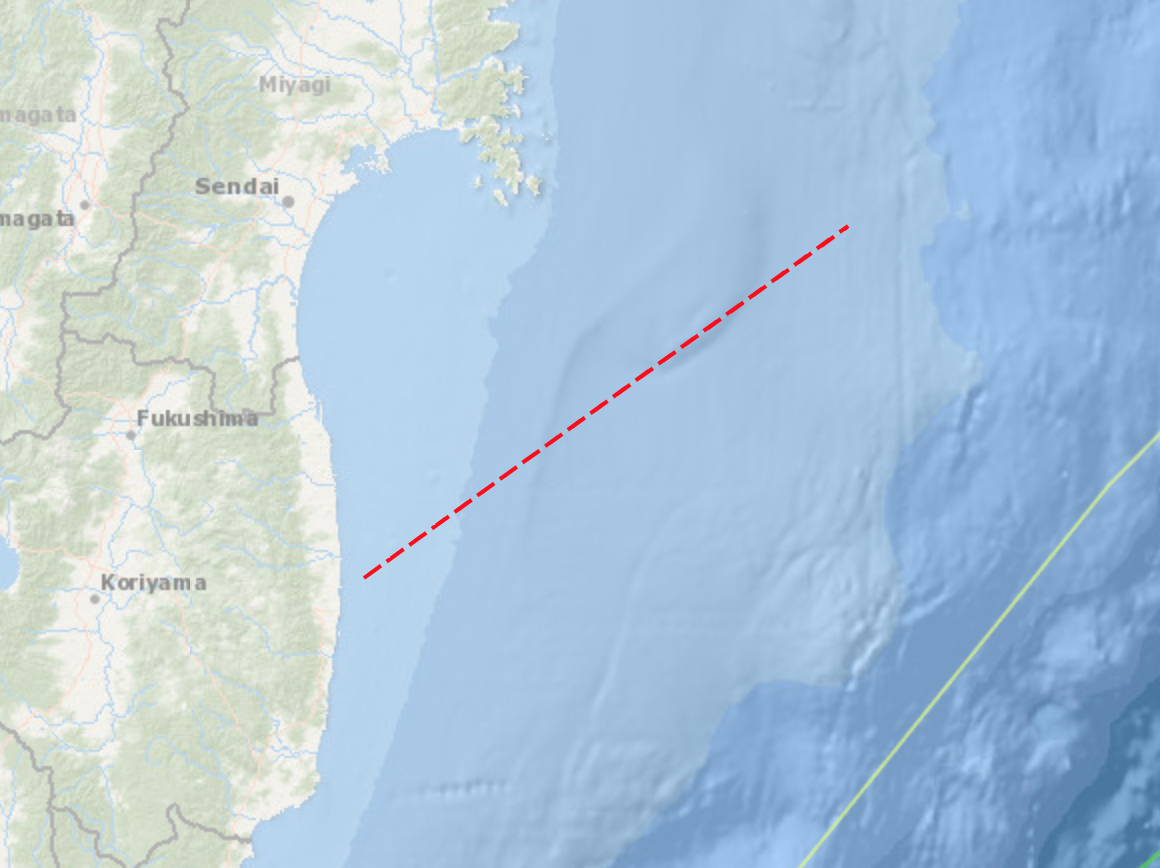
\includegraphics[scale=0.5]{1D.png}
\end{figure}
\noindent Using the control points, we can then apply the cubic B\'ezier curve to derive the following sea floor curve:
\begin{figure}[H]
\centering
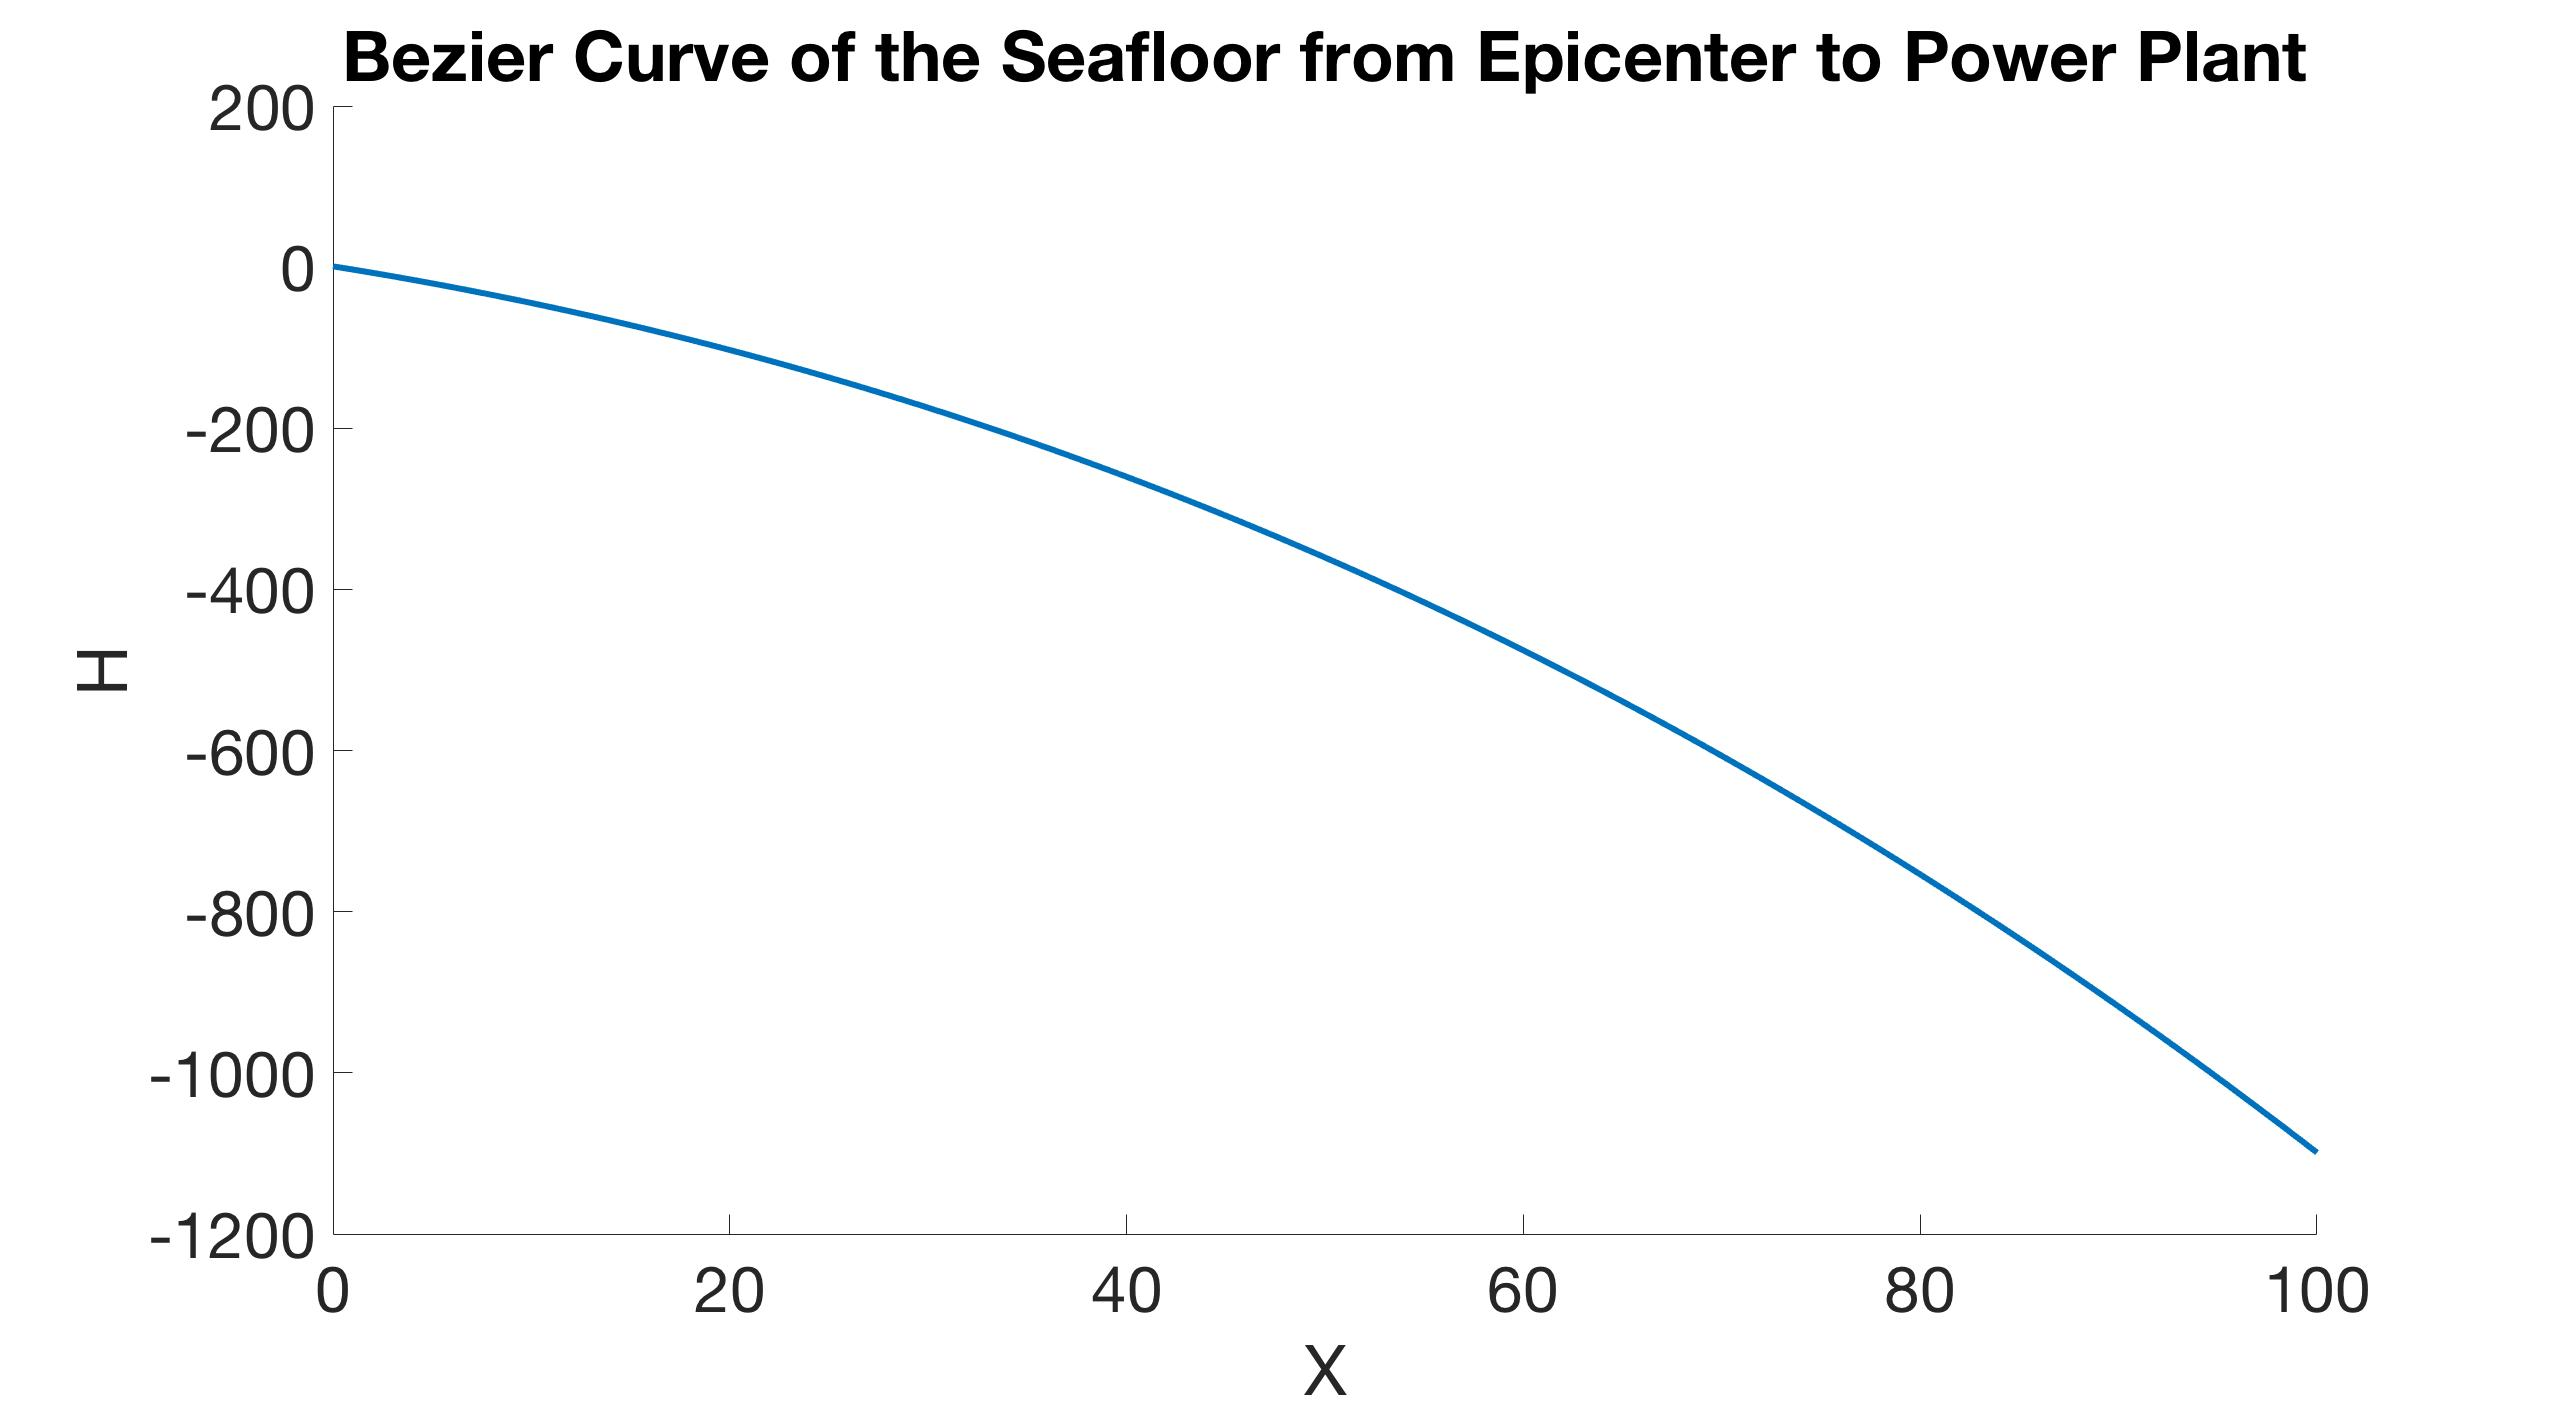
\includegraphics[scale=0.15]{1DLine.jpg}
\end{figure}
\noindent Similarly, we can also draw a rectangle with the diagonal being the line between the epicenter of the earthquake to the nuclear power plant.  This rectangle is then used to define the 16 control points in order to derive the 2D interpolated sea floor surface.
\begin{figure}[H]
\centering
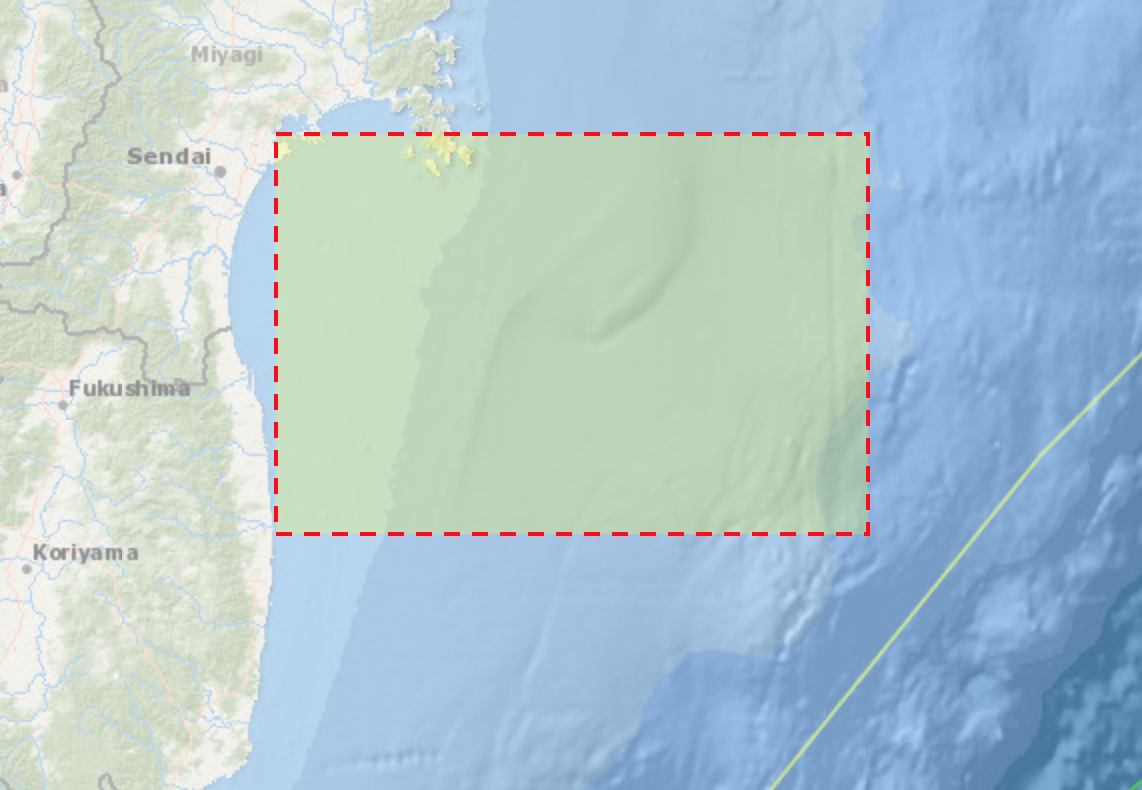
\includegraphics[scale=0.5]{2D.png}
\end{figure}
\noindent Using the control points, we linearly interpolate all the points within the grid, and derive the following sea floor.
\begin{figure}[H]
\centering
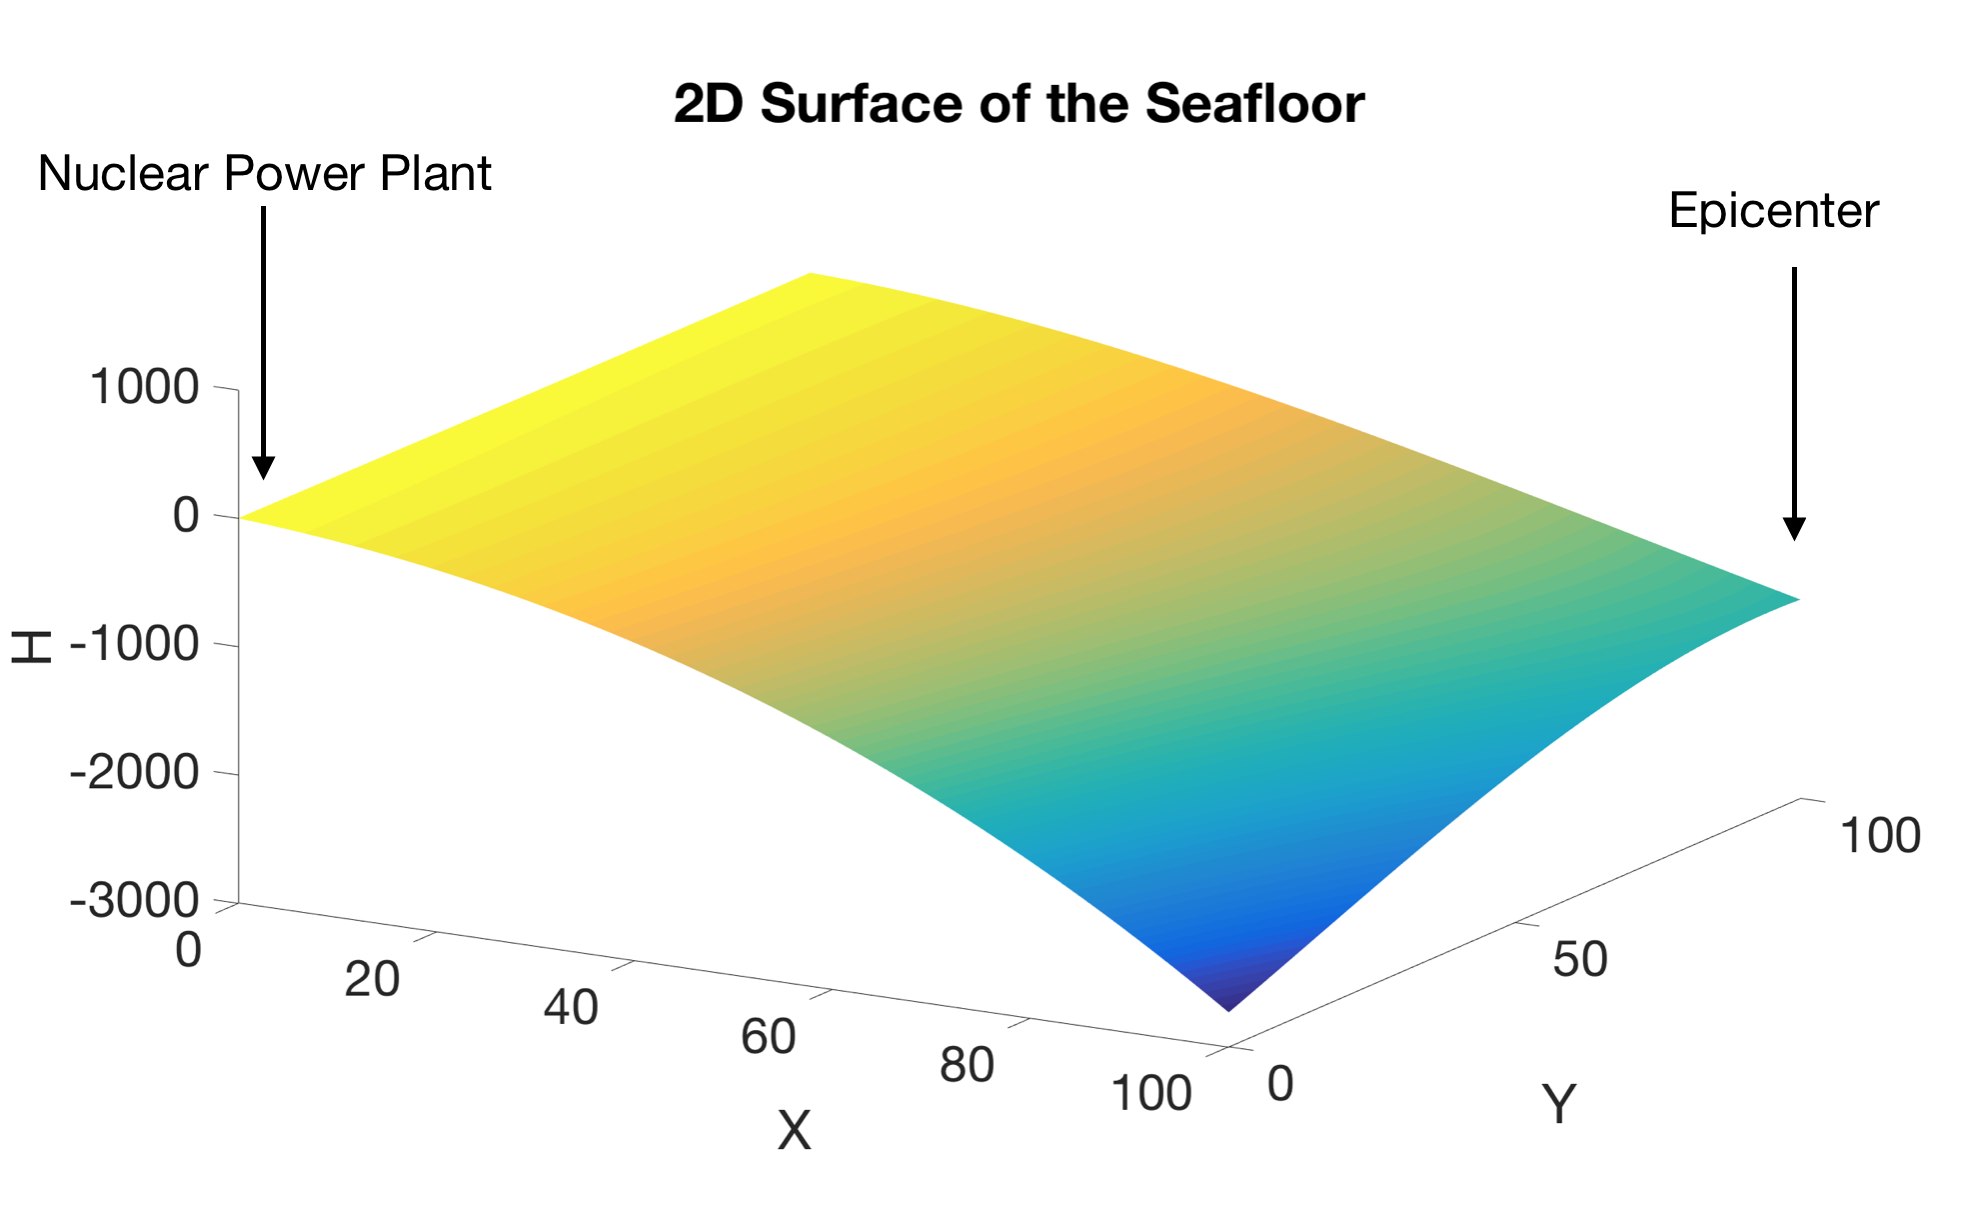
\includegraphics[scale=0.4]{2DSurf.png}
\end{figure}

\noindent The key benefit of using the B\'ezier cubic interpolation is that we can create approximations of the sea floor very easily with only a few defined points.  This gives us the liberty to apply our numerical method to any geographical location, and even test it with fictional surfaces. \\

%Following is what I (Lonny) added regarding the derivatives

\noindent Using Equation \ref{eq:bezierderiv} for the derivative at any point $t$, we now generate three-dimensional surface plots describing the partial derivatives with respect to $x$ and $y$ of the Bezier surface. These derivatives for $x$ and $y$ are stored in two matrices, each of size 100x100, where the $i$, $j$ element of each represents the partial derivative at $x$ location, $i$, and $y$ location, $j$. The images below are useful visual representations of these derivatives.

\begin{figure}[H]
\centering
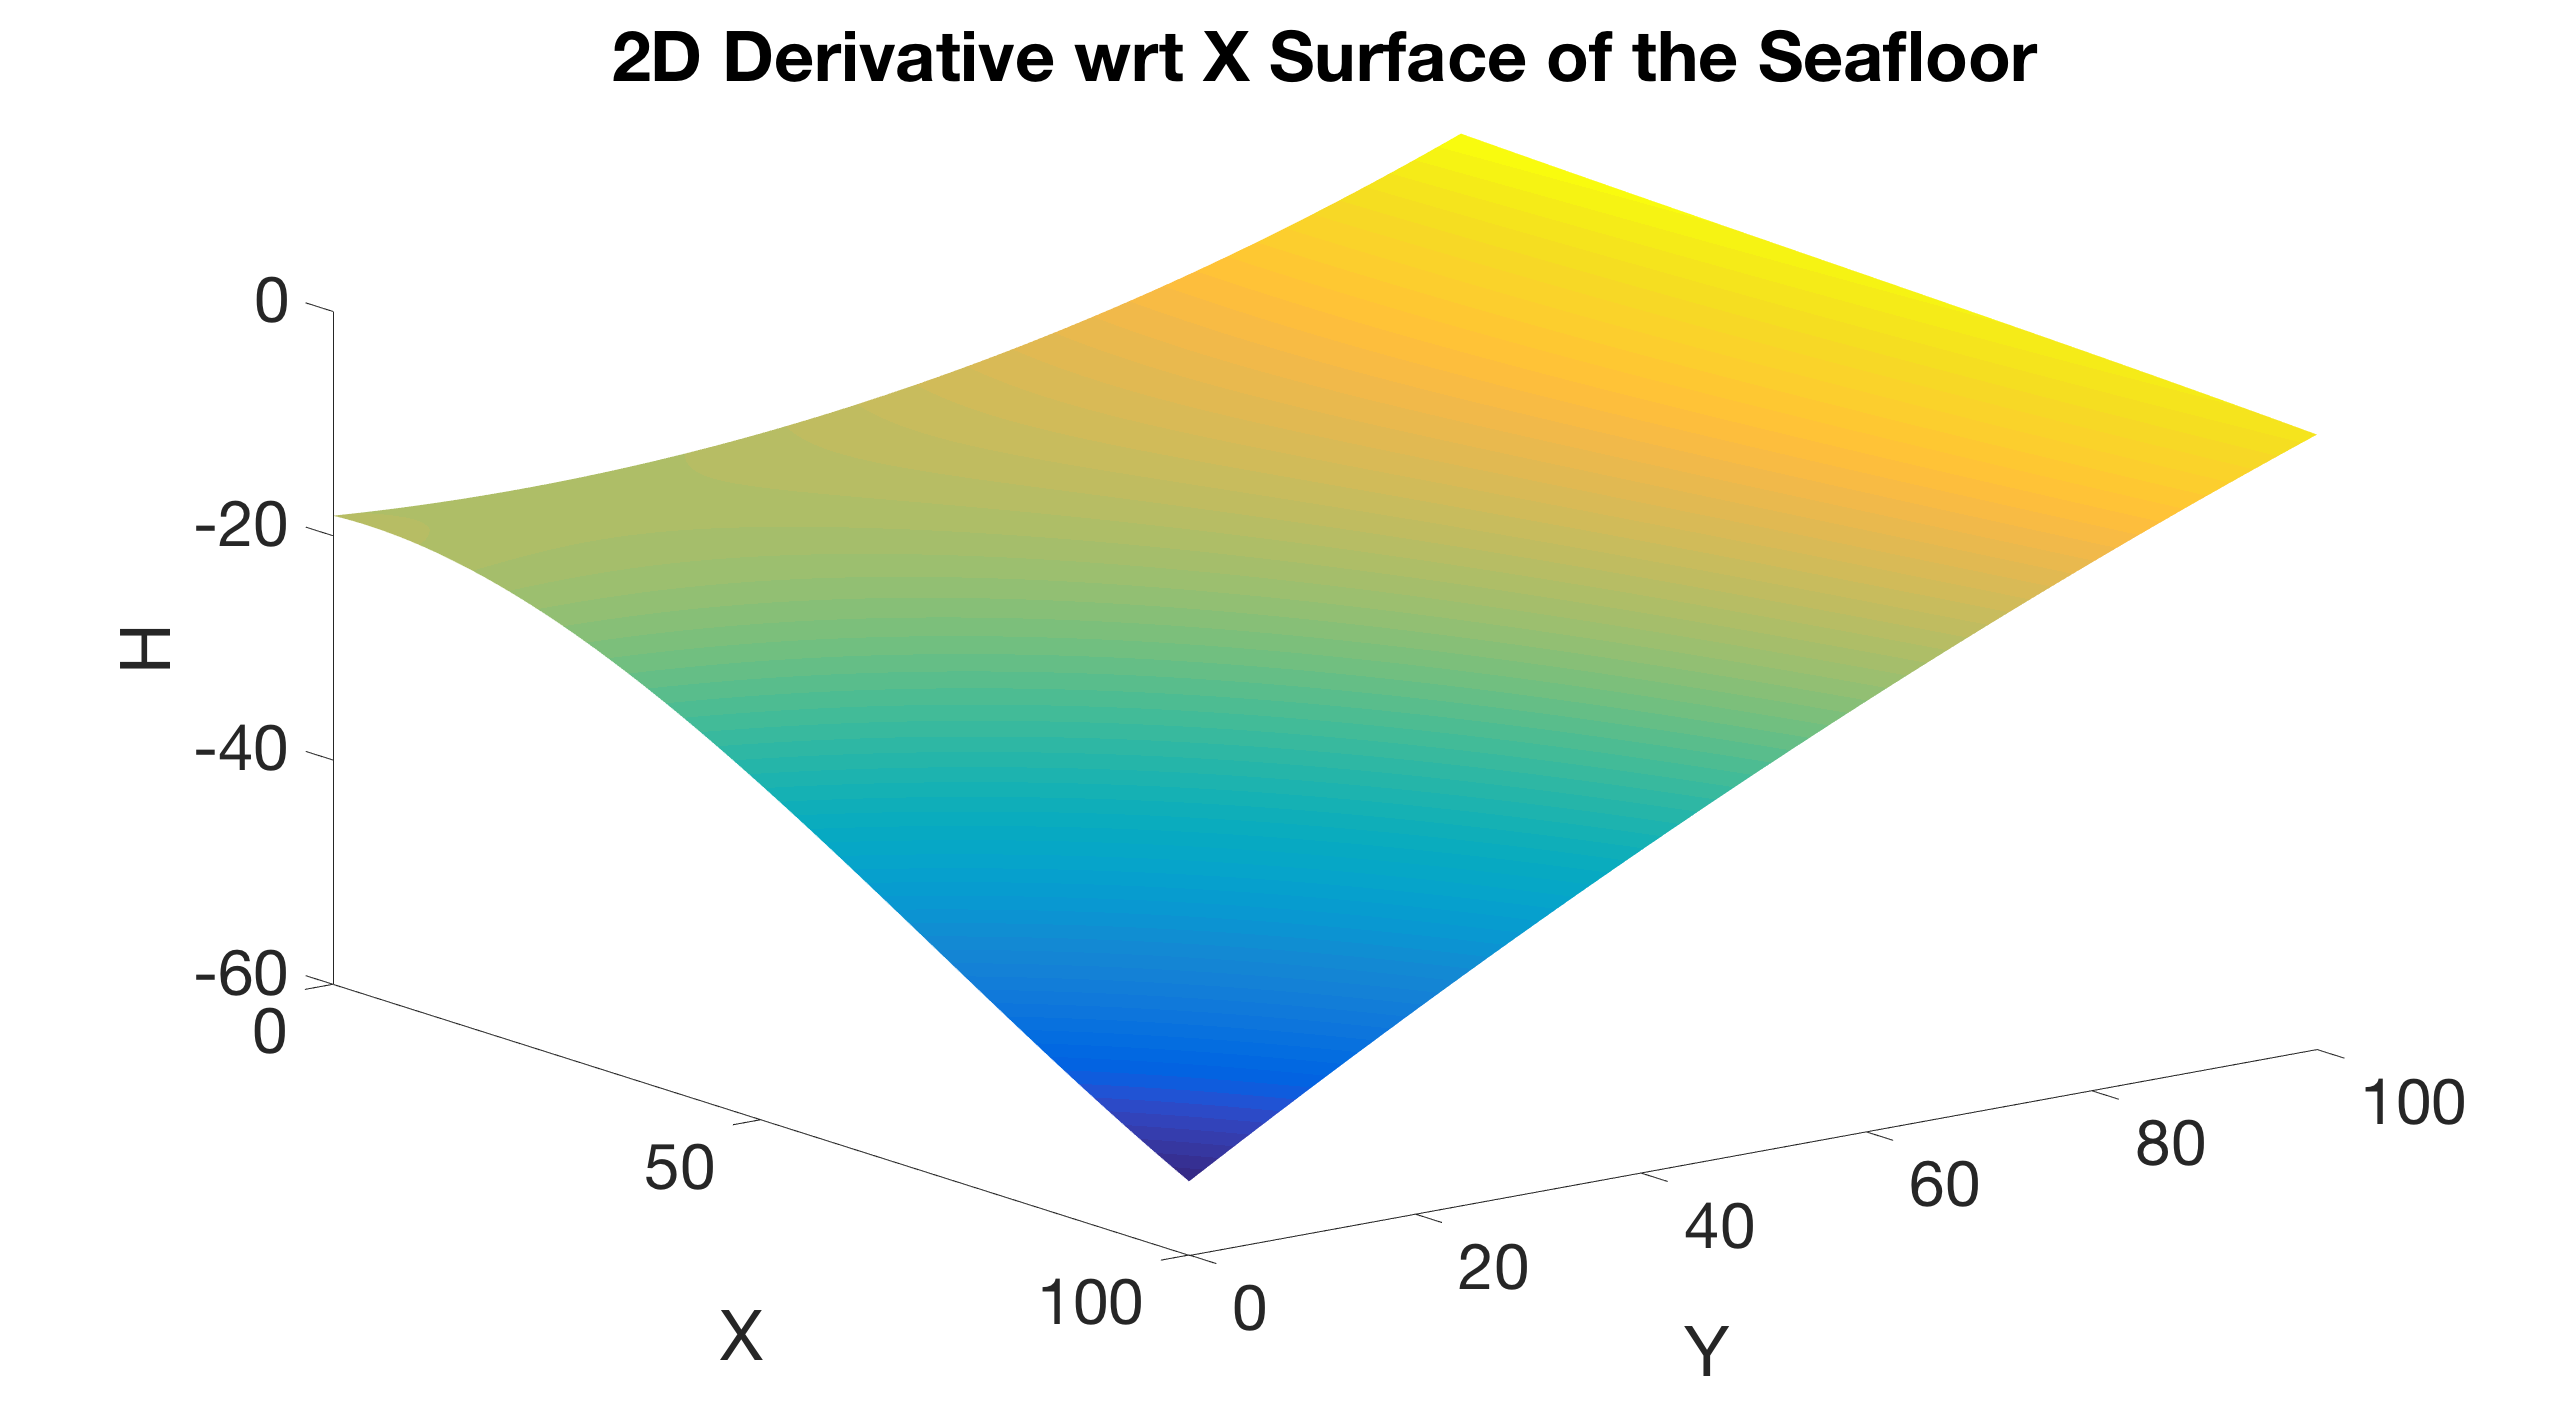
\includegraphics[scale=0.15]{SurfDerivX.png}
\caption{This is a surface plot of the derivative at each grid point with respect to $x$}
\end{figure}

\begin{figure}[H]
\centering
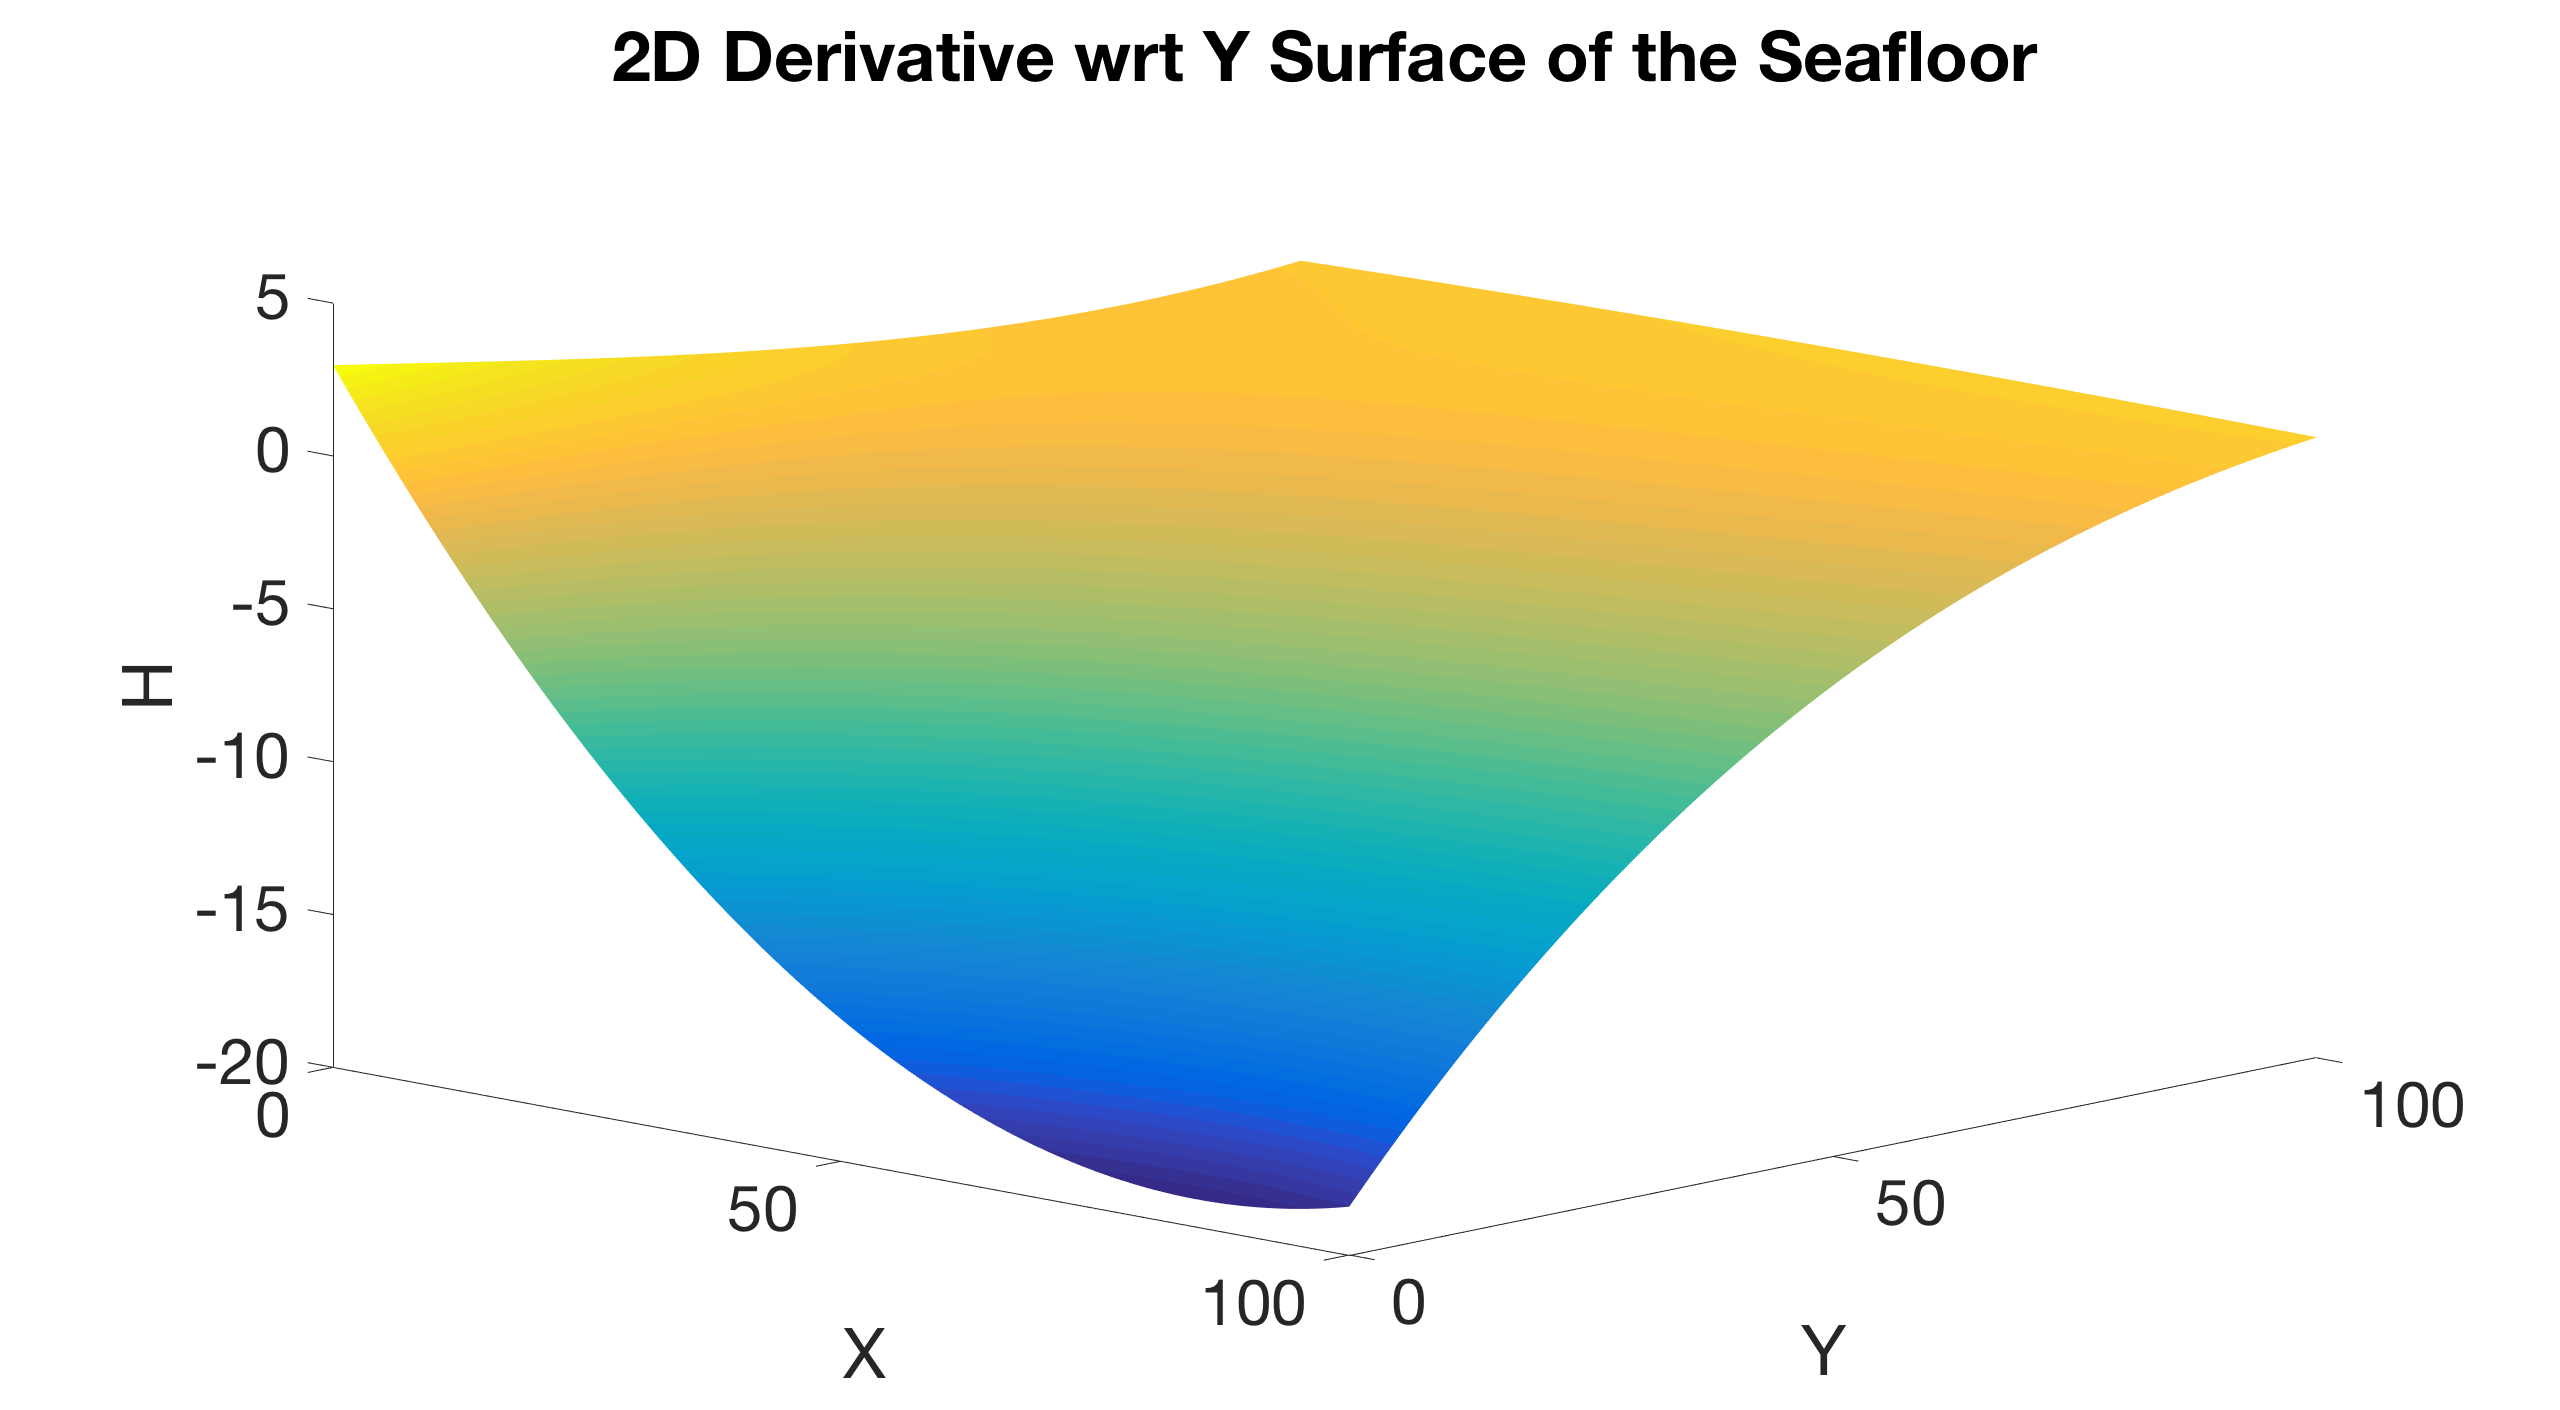
\includegraphics[scale=0.15]{SurfDerivY.png}
\caption{This is a surface plot of the derivative at each grid point with respect to $y$}
\end{figure}

\noindent These derivatives at each grid point are necessary for stepping forward in our model in order to better simulate the dynamics of the wave. This allows us to estimate the amplitude of the wave once reaching the nuclear power plant, which is assumed to be located a neglibible distance from the coast at which the elevation is set to the value 1 meter.

\end{document}
